Iš sinchronizuotų smegenų bangų duomenų\cite{brainwaves} rinkinio buvo pasirinktos dviejų asmenų duomenys.
Iškirptas tik tyrimo metu rodomos penkių minučių ilgumo vaizdo medžiagos metu užfiksuotos žemos gama bangos.
Vaizdo medžiagoje buvo užduotys tyrimo dalyviams, kurios turėtų įtakoti smegenų bangų veiklą, kaip aritmetis, nusiraminimas, mirksėjimas.
Žemos gama bangos yra siejamos su dėmesio reikalaujančia veikla, dėmesingumu.

\begin{figure}
    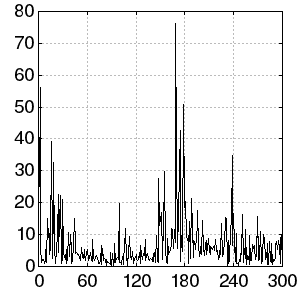
\includegraphics[scale=0.65]{../scripts/brainwaves/wave1.png}
    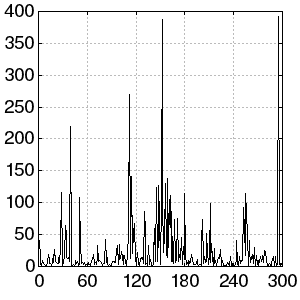
\includegraphics[scale=0.65]{../scripts/brainwaves/wave2.png}
    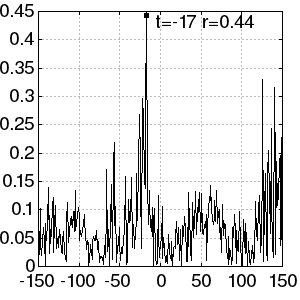
\includegraphics[scale=0.65]{../scripts/brainwaves/result.png}
    \caption{Grafikas kairėje: pirmo dalyvio žemos gama bangos. Grafikas centre: antro dalyvio gama bangos. Grafikas dešinėje: signalų tarpusavio koreliacija. Smegenų bangų signalo stiprumas \(y\) ašyje yra bedimencinis, pagal duomenis pateikusį šaltinį. Ašyje \(x\) - laikas sekundėmis}
    \label{fig:brainwaves}
\end{figure}

Signalų tarpusavio koreliacija turėtų būti stipriausia, kai \( t = 0 \), nes visi dalyviai vienu metu atlieka užduotis.
Bet iš grafiko (~\ref{fig:brainwaves} pav.) matome, kad dižiausias statistinis panašumas yra \( R_{fg}(t) = 0.44 \), kai \( t = -17 \).
Tokie rezultatai gali būti dėl tyrimo metu naudotos netikslios mėgėjiškos įrangos.
